% Компіляція: lualatex -shell-escape main.tex (двічі)
\documentclass[12pt,a4paper]{article}

\usepackage{fontspec}
\usepackage{polyglossia}
\setdefaultlanguage{ukrainian}
\setmainfont{NewComputerModern10}
\setsansfont{Noto Sans}
\setmonofont{Noto Sans Mono}[
  Scale=0.82,
  ItalicFont={Noto Sans Mono},
  ItalicFeatures={FakeSlant=0.2}
]

\usepackage{
  amsmath,
  amssymb,
  animate,
  array,
  booktabs,
  caption,
  enumitem,
  float,
  geometry,
  graphicx,
  microtype,
  titlesec,
  xcolor
}
\usepackage{tikz}
\usetikzlibrary{arrows.meta,positioning,shapes.geometric}
\geometry{left=2cm,right=2cm,top=2cm,bottom=2cm}
\setlength{\parindent}{1.25cm}
\setlength{\parskip}{0pt}
\linespread{1.08}
\titleformat{\section}
  {\normalfont\fontsize{14}{16}\selectfont\bfseries}
  {\thesection}{0.6em}{}
\titleformat{\subsection}
  {\normalfont\fontsize{12}{14}\selectfont\bfseries}
  {\thesubsection}{0.6em}{}
\titlespacing*{\section}{0pt}{1.4em}{0.65em}
\titlespacing*{\subsection}{0pt}{1.1em}{0.45em}
\captionsetup{font=small,labelfont=bf,labelsep=endash}
\captionsetup[table]{position=bottom,skip=5pt}
\setlist{itemsep=2pt,topsep=4pt}

\usepackage[newfloat]{minted}
\SetupFloatingEnvironment{listing}{name=Лістинг}
\setminted{%
  fontsize=\scriptsize,
  linenos,
  breaklines,
  breakanywhere,
  autogobble,
  frame=single,
  framesep=2mm,
  bgcolor=gray!5,
  tabsize=4
}

\usepackage[
  unicode,
  colorlinks=true,
  linkcolor=black,
  urlcolor=blue,
  pdftitle={ІО-41, Давидчук Артем, Інформаційне забезпечення промислових роботів, Лабораторна робота №3},
  pdfauthor={Давидчук Артем},
  pdfsubject={Програмування траєкторій руху робота-маніпулятора в імітаційному середовищі}
]{hyperref}

\begin{document}

\pagenumbering{gobble}
\begin{titlepage}
  \begin{center}
    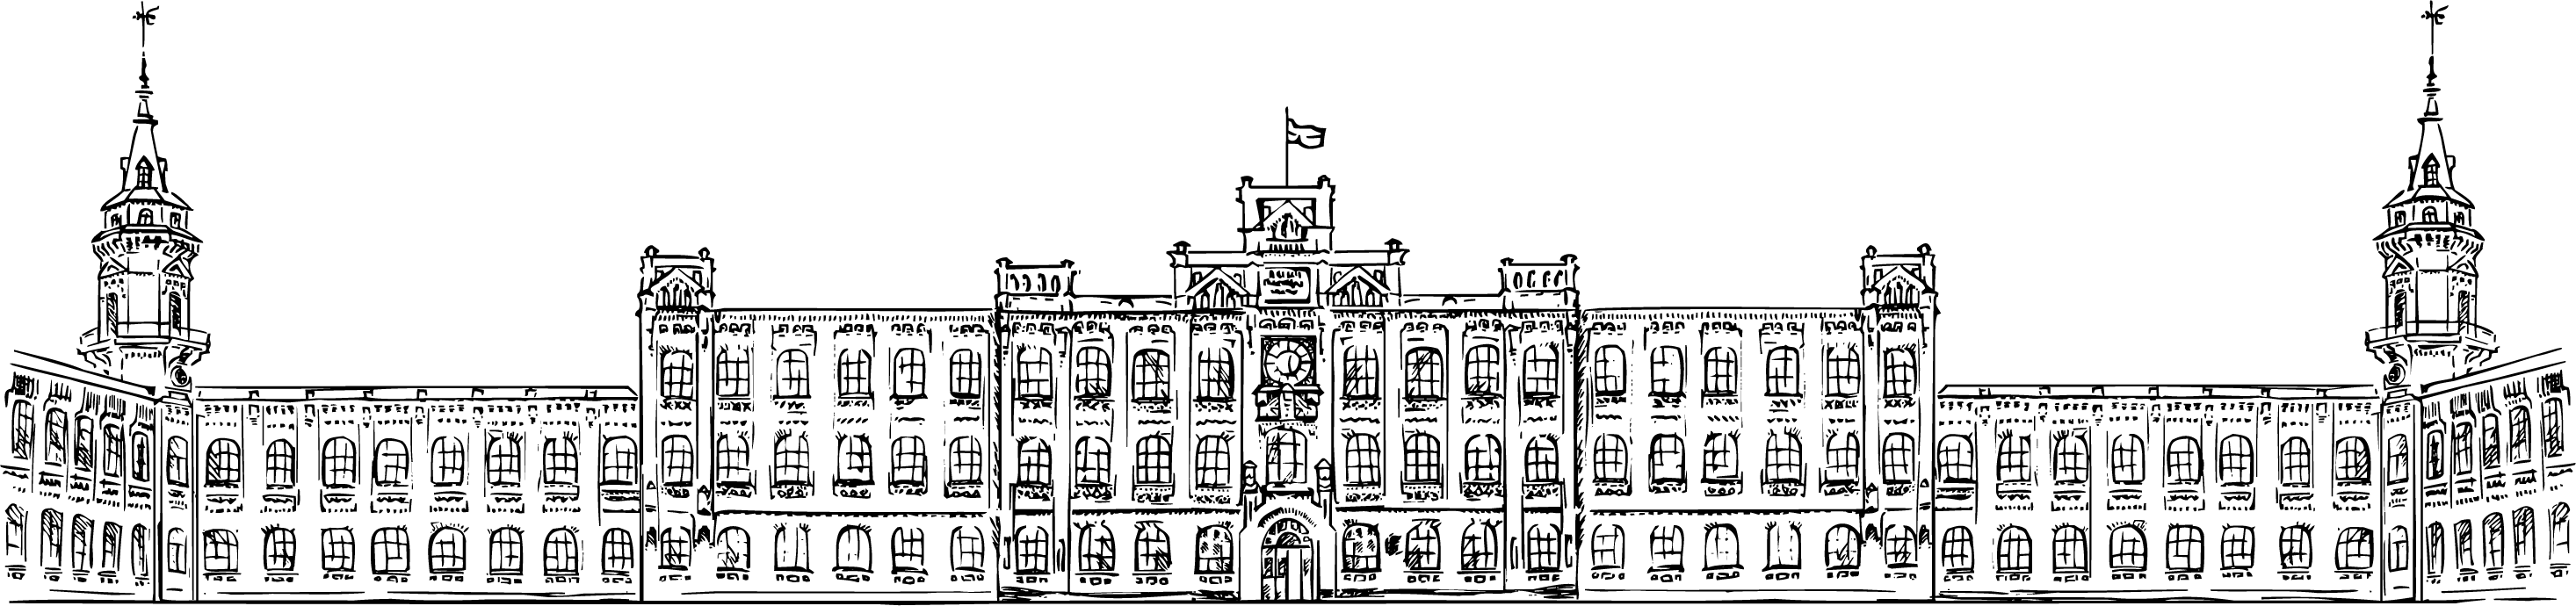
\includegraphics[width=0.7\textwidth]{../../../../../templates/letterhead.png}
  \end{center}

  \begin{center}
    \large
    Національний технічний університет України\\
    «Київський політехнічний інститут імені Ігоря Сікорського»\\[1em]
    Факультет інформатики та обчислювальної техніки\\
    Кафедра обчислювальної техніки
  \end{center}

  \vfill

  \begin{center}
    \textbf{\LARGE Інформаційне забезпечення\\промислових роботів}\\[2em]
    \textbf{\Large Лабораторна робота №3}\\[0.7em]
    \parbox{0.9\textwidth}{\centering
      «Програмування траєкторій руху робота-маніпулятора\\
      в імітаційному середовищі»}
  \end{center}

  \vfill

  \begin{flushright}
    \begin{minipage}{0.48\textwidth}
      Виконав: студент групи ІО-41\\
      \textit{Давидчук Артем}\\
      Варіант: 317\\[1em]
      Перевірив: \textit{Тюляков Дмитро Ігорович}
    \end{minipage}
  \end{flushright}

  \vfill

  \begin{center}Київ --- 2026\end{center}
\end{titlepage}
\pagenumbering{arabic}

\section{Мета роботи}

Отримати практичні навички моделювання роботизованої комірки та
програмування траєкторій руху промислових роботів у CoppeliaSim Edu.
Ознайомитися зі зворотною кінематикою, формуванням плавної траєкторії,
координацією двох маніпуляторів і застосуванням комп'ютерного зору для
визначення положення об'єкта.

\section{Завдання}

Розробити сцену, у якій на конвеєрі випадково з'являються червоні, зелені
та сині кульки. Перша роботизована рука повинна забирати кульку з конвеєра,
переносити її на проміжний стіл і повертатися у початкове положення.
Камера має визначати положення кульки, після чого друга рука повинна
перенести її до контейнера відповідного кольору та також повернутися у
початкове положення.

Необхідно забезпечити точне суміщення ефектора з кулькою, уникнути
зіткнення маніпуляторів, занурення ефектора всередину контейнера та
динамічного відскоку кульки після її відпускання.

\section{Опис роботизованої системи}

Роботизована комірка складається з двох моделей ABB IRB-140, конвеєра,
проміжного стола, камери та трьох контейнерів. Розподіл функцій між
елементами сцени наведено в табл.~\ref{tab:scene-components}.

\begin{table}[H]
  \centering
  \renewcommand{\arraystretch}{1.18}
  \begin{tabular}{|p{0.36\textwidth}|p{0.54\textwidth}|}
    \hline
    \textbf{Об'єкт сцени} & \textbf{Призначення} \\
    \hline
    \texttt{Picker1} & Перенесення кульки з конвеєра на проміжний стіл \\ \hline
    \texttt{Picker2} & Перенесення кульки зі стола до потрібного контейнера \\ \hline
    \texttt{ColorVisionSensor} & Пошук кольорової області та визначення координат її центра \\ \hline
    \texttt{Conveyor} & Зона подачі випадково створених кульок \\ \hline
    \texttt{RedBin}, \texttt{GreenBin}, \texttt{BlueBin} & Контейнери для кульок трьох кольорів \\ \hline
    \texttt{TwoRobotSortingController} & Керуючий Lua-сценарій і автомат станів \\ \hline
  \end{tabular}
  \caption{Основні компоненти сцени}
  \label{tab:scene-components}
\end{table}

Обидва маніпулятори працюють послідовно. Друга рука починає рух лише після
того, як перша завершила укладання кульки на стіл і повернулася додому.
Такий розподіл робочого часу усуває перетин траєкторій у центральній зоні.

\section{Математичні основи керування}

\subsection{Зворотна кінематика}

Положення та орієнтація ефектора відносно світової системи координат
визначаються добутком однорідних матриць перетворення:
\begin{equation}
  {}^{0}\!T_{e}
  ={}^{0}\!T_{1}\,{}^{1}\!T_{2}\cdots{}^{n-1}\!T_{e}
  =
  \begin{bmatrix}
    R & \mathbf{p} \\
    \mathbf{0}^{T} & 1
  \end{bmatrix},
\end{equation}
де \(R\) --- матриця орієнтації ефектора, а
\(\mathbf{p}=[x\ y\ z]^{T}\) --- його положення.

У сцені використано вбудований механізм зворотної кінематики CoppeliaSim.
Керуючий сценарій задає бажану позицію об'єкта \texttt{target}, а
IK-розв'язувач визначає вектор кутів суглобів
\(\mathbf{q}\), для якого
\begin{equation}
  f(\mathbf{q})=
  \begin{bmatrix}
    \mathbf{p}_{d} \\
    R_{d}
  \end{bmatrix}.
\end{equation}
Отже, у Lua-сценарії не потрібно безпосередньо обчислювати кути кожного
суглоба: достатньо формувати послідовність цільових точок ефектора.

\subsection{Формування плавної траєкторії}

Між початковою точкою \(\mathbf{p}_{0}\) і кінцевою точкою
\(\mathbf{p}_{1}\) використано інтерполяцію
\begin{equation}
  \mathbf{p}(t)=(1-s)\mathbf{p}_{0}+s\mathbf{p}_{1},
  \qquad
  s=3q^{2}-2q^{3},
  \qquad
  q=\min\left(1,\frac{t-t_{0}}{T}\right).
\end{equation}
Поліном \(3q^{2}-2q^{3}\) має нульову похідну на початку та наприкінці
інтервалу. Завдяки цьому ефектор розганяється і зупиняється плавно, без
різкої зміни швидкості.

\subsection{Визначення положення кульки}

Vision sensor формує RGB-зображення. Для кожного пікселя перевіряються
порогові умови кольору. Координати центра знайденої області обчислюються
як середнє арифметичне координат усіх \(N\) пікселів, що пройшли перевірку:
\begin{equation}
  x_{c}=\frac{1}{N}\sum_{i=1}^{N}x_{i},
  \qquad
  y_{c}=\frac{1}{N}\sum_{i=1}^{N}y_{i}.
\end{equation}

Для ортографічної камери перехід від піксельних координат до координат
робочої площини виконується лінійним масштабуванням:
\begin{equation}
  x_{w}=x_{0}+\left(\frac{x_{c}}{W}-\frac{1}{2}\right)L,
  \qquad
  y_{w}=y_{0}-\left(\frac{y_{c}}{H}-\frac{1}{2}\right)L,
\end{equation}
де \(W\) і \(H\) --- роздільна здатність сенсора,
\((x_{0},y_{0})\) --- центр поля огляду, \(L\) --- його розмір.

\section{Алгоритм роботи}

Керування реалізовано у вигляді автомата станів. Один цикл сортування
складається з таких етапів:
\begin{enumerate}
  \item створення кульки випадкового кольору та її рух по конвеєру;
  \item наближення \texttt{Picker1} до точки захвату;
  \item точне приєднання кульки до ефектора першої руки;
  \item перенесення кульки на стіл і повернення \texttt{Picker1} додому;
  \item пошук кульки камерою та обчислення її координат;
  \item захват кульки роботом \texttt{Picker2};
  \item перенесення до контейнера відповідного кольору;
  \item відпускання кульки над поверхнею контейнера;
  \item повернення \texttt{Picker2} у початкове положення.
\end{enumerate}

Послідовність переходів між станами системи показано на
рис.~\ref{fig:sorting-algorithm}.

\begin{figure}[H]
  \centering
  \begin{tikzpicture}[
    font=\footnotesize,
    node distance=4mm and 4mm,
    flow arrow/.style={-{Latex[length=2.5mm]},thick,draw=black!75},
    terminal/.style={
      draw=black!70,
      rounded corners=8pt,
      fill=black!5,
      align=center,
      text width=2.6cm,
      minimum height=11mm
    },
    process/.style={
      draw=black!70,
      rounded corners=2pt,
      fill=blue!5,
      align=center,
      text width=3.35cm,
      minimum height=13mm
    },
    vision/.style={process,fill=cyan!9},
    decision/.style={
      diamond,
      aspect=2.35,
      draw=black!70,
      fill=yellow!12,
      align=center,
      inner sep=1.5pt,
      text width=2.3cm
    },
    bin/.style={
      draw=black!70,
      rounded corners=2pt,
      align=center,
      text width=3.25cm,
      minimum height=11mm
    }
  ]
    \node[terminal] (start) {Початок циклу сортування};
    \node[process,right=of start] (spawn)
      {Створити кульку випадкового кольору};
    \node[process,right=of spawn] (conveyor)
      {Перемістити кульку конвеєром до зони захвату};
    \node[process,right=of conveyor] (pickone)
      {Сумістити \texttt{Picker1} з кулькою та виконати точний захват};

    \node[process,below=7mm of pickone] (table)
      {Перенести кульку на стіл і повернути \texttt{Picker1} додому};
    \node[vision,left=of table] (camera)
      {Знайти кульку камерою, обчислити координати та визначити колір};
    \node[process,left=of camera] (picktwo)
      {Сумістити \texttt{Picker2} з кулькою та виконати захват};
    \node[decision,below=8mm of camera] (colour) {Який колір кульки?};

    \node[bin,fill=red!9,below=7mm of colour,xshift=-4.2cm] (redbin)
      {Перемістити до \texttt{RedBin}};
    \node[bin,fill=green!10,below=7mm of colour] (greenbin)
      {Перемістити до \texttt{GreenBin}};
    \node[bin,fill=blue!9,below=7mm of colour,xshift=4.2cm] (bluebin)
      {Перемістити до \texttt{BlueBin}};

    \node[process,below=7mm of greenbin] (release)
      {Відпустити кульку над поверхнею обраного контейнера};
    \node[process,below=of release] (home)
      {Повернути \texttt{Picker2} у початкове положення};
    \node[terminal,below=of home] (finish) {Цикл завершено};

    \draw[flow arrow] (start) -- (spawn);
    \draw[flow arrow] (spawn) -- (conveyor);
    \draw[flow arrow] (conveyor) -- (pickone);
    \draw[flow arrow] (pickone) -- (table);
    \draw[flow arrow] (table) -- (camera);
    \draw[flow arrow] (camera) -- (picktwo);
    \draw[flow arrow] (picktwo.south) -- ++(0,-4mm) -| (colour.north);
    \draw[flow arrow] (colour.west) -| node[pos=0.25,above]{червона} (redbin.north);
    \draw[flow arrow] (colour.south) -- node[right]{зелена} (greenbin.north);
    \draw[flow arrow] (colour.east) -| node[pos=0.25,above]{синя} (bluebin.north);
    \draw[flow arrow] (redbin.south) |- (release.west);
    \draw[flow arrow] (greenbin) -- (release);
    \draw[flow arrow] (bluebin.south) |- (release.east);
    \draw[flow arrow] (release) -- (home);
    \draw[flow arrow] (home) -- (finish);
  \end{tikzpicture}
  \caption{Блок-схема алгоритму сортування кульки}
  \label{fig:sorting-algorithm}
\end{figure}

Захват реалізовано через тимчасове приєднання кульки до об'єкта
\texttt{tip}. Відносна позиція кульки примусово встановлюється у фіксоване
значення, тому між центром об'єкта й ефектором не накопичується похибка.
Після сортування кулька від'єднується та встановлюється у визначену точку
контейнера як статичний об'єкт. Це усуває відскок і зависання.

\section{Програмна реалізація}

Керуючий сценарій написано мовою Lua. Повний код розміщено у файлі
\nolinkurl{cw3_v317_two_robot_sorting.lua}. Нижче наведено ключові
фрагменти реалізації.

\subsection{Плавне переміщення цільової точки}

\begin{listing}[H]
\begin{minted}{lua}
local function startMove(target, position, duration)
    moveFrom = sim.getObjectPosition(target, sim.handle_world)
    moveTo = position
    moveTime = duration
    t0 = sim.getSimulationTime()
end

local function updateMove(target)
    local q = math.min(1, (sim.getSimulationTime() - t0) / moveTime)
    local s = q * q * (3 - 2 * q)
    local p = {
        moveFrom[1] + (moveTo[1] - moveFrom[1]) * s,
        moveFrom[2] + (moveTo[2] - moveFrom[2]) * s,
        moveFrom[3] + (moveTo[3] - moveFrom[3]) * s
    }
    sim.setObjectPosition(target, sim.handle_world, p)
    return q >= 1
end
\end{minted}
\caption{Інтерполяція положення ефектора}
\end{listing}

\subsection{Точний захват і відпускання кульки}

\begin{listing}[H]
\begin{minted}{lua}
-- Захват першою рукою
sim.setObjectParent(ball, tip1, false)
sim.setObjectPosition(ball, tip1, {0, 0, -0.06})

-- Укладання на проміжний стіл
sim.setObjectParent(ball, -1, true)
sim.setObjectPosition(
    ball,
    sim.handle_world,
    {tablePosition[1], tablePosition[2], 0.105}
)
startMove(p1, home1, 1.0)

-- Укладання в контейнер і повернення другої руки
sim.setObjectParent(ball, -1, true)
sim.setObjectPosition(ball, sim.handle_world, binPositions[colorName])
startMove(p2, home2, 1.0)
\end{minted}
\caption{Захват, позиціювання та повернення маніпуляторів}
\end{listing}

\subsection{Виділення кольорової області}

\begin{listing}[H]
\begin{minted}{lua}
for y = 0, h - 1 do
    for x = 0, w - 1 do
        if x > w * 0.30 and x < w * 0.70
           and y > h * 0.30 and y < h * 0.70 then
            local i = (y * w + x) * 3 + 1
            local r, g, b = data[i], data[i + 1], data[i + 2]
            local c = nil

            if r > 190 and g < 110 and b < 110 then
                c = 'red'
            elseif g > 150 and r < 130 and b < 150 then
                c = 'green'
            elseif b > 170 and r < 130 and g < 170 then
                c = 'blue'
            end

            if c then
                sums[c][1] = sums[c][1] + x
                sums[c][2] = sums[c][2] + y
                counts[c] = counts[c] + 1
            end
        end
    end
end
\end{minted}
\caption{Порогова класифікація пікселів зображення}
\end{listing}

Після обчислення центра кольорової області камера передає координати
ефектору другої руки. Колір області звіряється з міткою створеного об'єкта,
щоб помаранчеві деталі роботів, які частково потрапляють у кадр, не
спричиняли хибного вибору контейнера.

\section{Результати виконання}

У результаті створено працездатну роботизовану комірку з двома
маніпуляторами, конвеєром, проміжним столом, камерою та трьома контейнерами.
Загальний вигляд змодельованої сцени наведено на
рис.~\ref{fig:scene-result}. Реалізована система послідовно передає кульку
між маніпуляторами, визначає її колір і розміщує у відповідному контейнері.

\begin{figure}[H]
  \centering
  \animategraphics[
    autoplay,
    loop,
    width=0.82\textwidth,
    poster=first
  ]{50}{lab3_frames_side_50fps_fast_q80/report-}{000}{302}
  \caption{Робота двох маніпуляторів у CoppeliaSim Edu}
  \label{fig:scene-result}
\end{figure}

Результати перевірки основних вимог наведено в
табл.~\ref{tab:results}.

\begin{table}[H]
  \centering
  \renewcommand{\arraystretch}{1.08}
  \begin{tabular}{|p{0.68\textwidth}|c|}
    \hline
    \textbf{Перевірена функція} & \textbf{Результат} \\
    \hline
    Випадкова генерація кульок трьох кольорів & Виконано \\ \hline
    Перенесення кульки першою рукою на стіл & Виконано \\ \hline
    Повернення першої руки у початкове положення & Виконано \\ \hline
    Визначення положення кульки камерою & Виконано \\ \hline
    Сортування кульки у відповідний контейнер & Виконано \\ \hline
    Повернення другої руки у початкове положення & Виконано \\ \hline
    Відсутність зіткнення рук і відскоку кульки & Виконано \\ \hline
  \end{tabular}
  \caption{Результати перевірки сцени}
  \label{tab:results}
\end{table}

\section{Висновок}

У лабораторній роботі створено комірку з двома маніпуляторами ABB IRB-140,
конвеєром, столом, камерою та трьома контейнерами. Реалізовано плавний
траєкторний рух, зворотну кінематику, пошук кольорової області та послідовний
автомат станів. Примусове суміщення кульки з ефектором забезпечило точний
захват, статичне позиціювання усунуло відскок, а повернення маніпуляторів у
початкові положення запобігло зіткненням. Поставлене завдання виконано
повністю.

\end{document}
